\documentclass[a4paper,12pt]{article}
\usepackage[brazil, english]{babel}
\usepackage[utf8]{inputenc}
\usepackage[T1]{fontenc}
\usepackage{geometry}
\usepackage{setspace}
\usepackage{titlesec}
\usepackage{hyperref}
\usepackage{graphicx}
\usepackage{caption}
\usepackage{subcaption}
\usepackage{fancyhdr}
\setlength{\headheight}{15pt}
\addtolength{\topmargin}{-2.5pt}
\usepackage{xcolor}
\usepackage{amsmath, amssymb, bm}
\usepackage{mathtools}
\usepackage{cancel}
\usepackage{tikz}
\usepackage{newunicodechar}
\usepackage{ragged2e}
\usepackage{setspace}
\usepackage{tikz-3dplot} % Necessário para coordenadas 3D
\usetikzlibrary{intersections}
\usepackage{siunitx}
\usetikzlibrary{3d, arrows.meta}
\usepackage{booktabs}

\usepackage{color}
\definecolor{myblue}{rgb}{.8, .8, 1}

\definecolor{ao(english)}{rgb}{0.0, 0.5, 0.0}

\usepackage{amsmath}
\usepackage{empheq}

\newlength\mytemplen
\newsavebox\mytempbox

\makeatletter
\newcommand\mybluebox{%
    \@ifnextchar[%]
       {\@mybluebox}%
       {\@mybluebox[0pt]}}

\def\@mybluebox[#1]{%
    \@ifnextchar[%]
       {\@@mybluebox[#1]}%
       {\@@mybluebox[#1][0pt]}}

\def\@@mybluebox[#1][#2]#3{
    \sbox\mytempbox{#3}%
    \mytemplen\ht\mytempbox
    \advance\mytemplen #1\relax
    \ht\mytempbox\mytemplen
    \mytemplen\dp\mytempbox
    \advance\mytemplen #2\relax
    \dp\mytempbox\mytemplen
    \colorbox{myblue}{\hspace{1em}\usebox{\mytempbox}\hspace{1em}}}
\makeatother

\usepackage[most]{tcolorbox}

\newtcbox{\mymath}[1][]{%
    nobeforeafter, math upper, tcbox raise base,
    enhanced, colframe=blue!30!black,
    colback=blue!30, boxrule=1pt,
    #1}

\tcbset{
    highlight math style={
        enhanced,
        colframe=red!60!black,
        colback=yellow!50,
        arc=4pt,
        boxrule=1pt,
        drop fuzzy shadow
    }
    }

\usepackage{physics}
\usepackage{pgfplots}
\pgfplotsset{compat=1.17}

\linespread{1.5}

\definecolor{ao(english)}{rgb}{0.0, 0.5, 0.0}
\definecolor{byzantium}{rgb}{0.44, 0.16, 0.39}
\newunicodechar{∘}{\circ}

%%%%%%%%%%%%%%%%%%%%%%%%%%%%%%%%%%%%%%%%%%%%%%%%%%
% These are some new commands that may be useful 
% for paper writing in general. If other new commands
% are needed for your specific paper, please feel 
% free to add here. 
%
% The currently available commands are organized in: 
% 1) Systems
% 2) Quantities
% 3) Energies and units
% 4) particle species
% 5) Colors package
% 6) hyperlink
%%%%%%%%%%%%%%%%%%%%%%%%%%%%%%%%%%%%%%%%%%%%%%%%%%

\usepackage{amsmath}
\usepackage{amssymb}
\usepackage{upgreek}
\usepackage{multirow}
\usepackage{setspace}% http://ctan.org/pkg/setspace
\usepackage{fancyhdr}
\usepackage{datetime}

% 1) SYSTEMS
\newcommand{\btc}               {\textbf{BTC}}
\newcommand{\btcspace}          {\textbf{BTC} }
\newcommand{\pow}               {\textbf{PoW}}

% 4) definition to references, biblatex and hyperlink
\usepackage[backend=bibtex, 
style=nature,  %style reference.
sorting=none,
firstinits=true %first name abbreviate
]{biblatex}

\usepackage{hyperref}
\hypersetup{
    colorlinks=true, %set "true" if you want colored links
    linktoc=all,     %set to "all" if you want both sections and subsections linked
    linkcolor=blue,  %choose some color if you want links to stand out
    citecolor= blue, % color of \cite{} in the text.
    urlcolor  = blue, % color of the link for the paper in references.
}

% 5) Tikz and figures
\usepackage{epsfig}
\usepackage{lmodern}
\usepackage{mathtools}
\usepackage[utf8]{luainputenc}
\usepackage{xspace}
\usepackage{tikz}
\usepackage{pgfplots}
\pgfplotsset{compat=newest}

\usetikzlibrary{positioning}
\usepackage{subcaption}

% 6) colors:
\usepackage{xcolor}
\definecolor{ao(english)}{rgb}{0.0, 0.5, 0.0} % dark green

% 7) Add lines numbers
%\usepackage{lineno}

% add pdf file to thesis:
\usepackage{pdfpages}

\hypersetup{
    colorlinks=true,% make the links colored
    linkcolor=blue
}

\usepackage{setspace}
\addbibresource{bibliography.bib}

\newcommand{\printingbibliography}{%

    \pagestyle{myheadings}
    \markright{}
    \sloppy
    \printbibliography[heading=bibintoc, % add to table of contents
                   title=Refer\^encias % Chapter name
                  ]
    \fussy%
}
\PassOptionsToPackage{table}{xcolor}

\pagestyle{fancy}
\fancyhf{}
\renewcommand{\headrulewidth}{0pt}
\fancyhead[R]{\thepage}

\geometry{a4paper,top=30mm,bottom=20mm,left=30mm,right=20mm}

\titleformat*{\section}{\bfseries\large}
\titleformat*{\subsection}{\bfseries\normalsize}

\title{Concurso Público do Instituto Federal de Sergipe para provimento dos cargos
efetivos de Professor do EBTT \textbf{\large F\'isica}.}
\author{Andr\'e V. Silva \\ \texttt{\url{www.andrevsilva.com}}}
\date{\today}

\begin{document}

\maketitle
\noindent\rule{\linewidth}{0.4pt}\\

\justifying
\colorbox{yellow!30}{A Terra não é um referencial inercial porque ela tem movimentos acelerados}, como a rotação em torno de seu eixo 
e a translação em torno do Sol. Esses movimentos geram \colorbox{yellow!30}{forças fictícias (como Coriolis e centrífuga)} que só existem em referenciais não inerciais.

Cálculo da aceleração centrípeta de um ponto na superfície da Terra devido à rotação:

\begin{itemize}
  \item Raio da Terra: \( R \approx 6,37 \times 10^6 \, \mathrm{m} \)
  \item Período de rotação: \( T = 24 \, \mathrm{h} = 86400 \, \mathrm{s} \)
\end{itemize}

\textbf{Passo 1: velocidade angular}
\[
\omega = \frac{2\pi}{T} \approx \frac{2\pi}{86400} \approx 7,27 \times 10^{-5} \, \mathrm{rad/s}
\]

\textbf{Passo 2: aceleração centrípeta}
\[
a_c = \omega^2 R
\]

Substituindo os valores numéricos:
\[
a_c = \bigl(7,27 \times 10^{-5}\bigr)^2 \cdot 6,37 \times 10^6
\]

\[
a_c \approx 0,034 \, \mathrm{m/s}^2
\]

\textbf{Resultado:}
\[
\boxed{a_c \approx 0,034 \, \mathrm{m/s}^2}
\]

\begin{flushleft}
\textbf{\textcolor{blue}{\Large Q31}}\\
\noindent
A \colorbox{yellow}{1ª Lei de Newton do Movimento, ou Lei da Inércia}, define 
os referenciais inerciais e os referenciais não inerciais. \colorbox{green!40}{A 
Terra não é um referencial inercial porque possui}

\begin{itemize}
\item[(A)] massa maior que a massa da Lua.
\item[(B)] movimento de rotação em torno do seu eixo.
\item[(C)] superfície irregular, com deformações.
\item[(D)] massa menor que a massa do Sol.
\end{itemize}

\vspace{0.5cm}

\textcolor{red}{\textbf{Solução:}}\\

A resposta correta é alternativa \colorbox{green!50}{\textbf{B}}.
\end{flushleft}

\noindent\rule{\linewidth}{0.6pt}\\

\section*{As Leis de Newton – Leis Fundamentais da Mecânica}

Isaac Newton formulou, no século XVII, três princípios fundamentais que descrevem as relações entre as forças aplicadas a um corpo e o movimento que ele executa. Essas leis são a base da Mecânica Clássica.

\subsection*{1ª Lei de Newton – Lei da Inércia}

\textbf{``Todo corpo continua em seu estado de repouso ou de movimento retilíneo uniforme, a menos que seja obrigado a mudar esse estado por forças que sobre ele atuem.''}

Em outras palavras: um corpo tende a manter sua velocidade constante (em módulo, direção e sentido) se a força resultante sobre ele for nula. Isso significa que a tendência natural dos corpos não é ``parar'' (como pensavam os gregos), mas sim manter o estado em que estão, seja parado, seja em movimento retilíneo uniforme.

Matematicamente:
\[
\sum \vec{F} = 0 \implies \vec{v} = \text{constante}
\]

\subsection*{2ª Lei de Newton – Princípio Fundamental da Dinâmica}

\textbf{``A força resultante sobre um corpo é igual ao produto da sua massa pela aceleração que ele adquire.''}

Em outras palavras: quando a força resultante sobre um corpo é diferente de zero, ele sofre uma aceleração na mesma direção e sentido da força resultante.

Matematicamente:
\[
\sum \vec{F} = m \vec{a}
\]

onde:
\begin{itemize}
    \item \( \sum \vec{F} \): força resultante sobre o corpo
    \item \( m \): massa do corpo (constante)
    \item \( \vec{a} \): aceleração do corpo
\end{itemize}

Essa lei também pode ser interpretada como a relação de causa (força resultante) e efeito (aceleração).

\subsection*{3ª Lei de Newton – Princípio da Ação e Reação}

\textbf{``A toda ação corresponde sempre uma reação, de mesma intensidade, mesma direção e sentido oposto.''}

Em outras palavras: sempre que um corpo \( A \) exerce uma força sobre um corpo \( B \), o corpo \( B \) exerce uma força de mesma intensidade e direção, mas em sentido oposto, sobre o corpo \( A \).

Matematicamente:
\[
\vec{F}_{AB} = -\vec{F}_{BA}
\]

Essas forças:
\begin{itemize}
    \item nunca se anulam entre si, pois atuam em corpos diferentes;
    \item sempre ocorrem em pares (ação e reação simultaneamente).
\end{itemize}

\subsection*{Resumo}

\begin{center}
\begin{tabular}{lll}
\toprule
\textbf{Lei} & \textbf{Nome} & \textbf{Fórmula} \\
\midrule
1ª & Inércia & \( \sum \vec{F} = 0 \implies \vec{v} = \text{constante} \) \\
2ª & Dinâmica & \( \sum \vec{F} = m \vec{a} \) \\
3ª & Ação e Reação & \( \vec{F}_{AB} = -\vec{F}_{BA} \) \\
\bottomrule
\end{tabular}
\end{center}

\noindent\rule{\linewidth}{0.6pt}\\

\begin{flushleft}
\textbf{\textcolor{blue}{\Large Q32}}\\
\noindent

Um bloco \(A\) de massa \(m_1\) está sobre uma mesa horizontal.  
O coeficiente de atrito cinético entre o bloco e a mesa é \(\mu_k\).  
Um fio inextensível e de massa desprezível, conectado ao bloco \(A\), passa por uma polia de massa e atrito desprezíveis.  
Na outra extremidade do fio, está um bloco \(B\) de massa \(m_2\), suspenso.  
Quando o bloco \(A\) desliza sobre a mesa, puxado pelo bloco \(B\), a tensão no fio é igual a:


\begin{itemize}
\item[(A)] $\quad \frac{m_1 m_2 (1 + \mu_k) g}{m_1 + m_2}
\qquad$
\item[(B)] $\quad \frac{(m_2 + \mu_k m_1) g}{m_1 + m_2}\qquad$
\item[(C)] $\quad \frac{m_1 m_2 (1 - \mu_k) g}{m_1 + m_2}
\qquad$
\item[(D)] $\quad \frac{(m_2 - \mu_k m_1) g}{m_1 + m_2}$
\end{itemize}

\vspace{0.5cm}


\textcolor{red}{\textbf{Solução:}}\\

Queremos determinar a \textbf{tensão \( T \)} no fio.

\subsection*{Análise das forças}

\subsubsection*{Bloco \( A \) (horizontal)}
Forças horizontais no bloco \( A \):
\[
T - f_{\text{at}} = m_1 a
\]

O atrito cinético é dado por:
\[
f_{\text{at}} = \mu_k m_1 g
\]

Portanto:
\[
T - \mu_k m_1 g = m_1 a
\]

\[
T = m_1 a + \mu_k m_1 g
\]

\subsubsection*{Bloco \( B \) (vertical)}
Forças verticais no bloco \( B \):
\[
m_2 g - T = m_2 a
\]

\subsection*{Equação do sistema}

Os blocos têm aceleração comum \( a \). Somamos as equações:
\[
(T - \mu_k m_1 g) + (m_2 g - T) = m_1 a + m_2 a
\]

O termo \( T \) se cancela:
\[
m_2 g - \mu_k m_1 g = (m_1 + m_2) a
\]

Assim:
\[
\boxed{
a = \frac{m_2 g - \mu_k m_1 g}{m_1 + m_2}
}
\]

\subsection*{Substituindo \( a \) em \( T \)}

Substituímos \( a \) na equação do bloco \( A \):
\[
T = m_1 a + \mu_k m_1 g
\]

\[
T = m_1 \cdot \frac{m_2 g - \mu_k m_1 g}{m_1 + m_2} + \mu_k m_1 g
\]

Distribuindo:
\[
T = \frac{m_1 m_2 g - \mu_k m_1^2 g}{m_1 + m_2} + \frac{\mu_k m_1 g (m_1 + m_2)}{m_1 + m_2}
\]

Somamos os termos:
\[
T = \frac{m_1 m_2 g - \mu_k m_1^2 g + \mu_k m_1^2 g + \mu_k m_1 m_2 g}{m_1 + m_2}
\]

Os termos \( -\mu_k m_1^2 g + \mu_k m_1^2 g \) se cancelam:
\[
T = \frac{m_1 m_2 g + \mu_k m_1 m_2 g}{m_1 + m_2}
\]

Fatorando:
\[
T = \frac{m_1 m_2 g (1 + \mu_k)}{m_1 + m_2}
\]

\subsection*{Resposta final:}
\[
\boxed{
T = \frac{m_1 m_2 g (1 + \mu_k)}{m_1 + m_2}
}
\]

A resposta correta é alternativa \colorbox{green!50}{\textbf{A}}.


\end{flushleft}

\noindent\rule{\linewidth}{0.6pt}\\


\begin{flushleft}
\textbf{\textcolor{blue}{\Large Q33}}\\
\noindent
Num plano inclinado com atrito, que faz um ângulo $\theta$ com
uma superfície horizontal, está uma esfera em repouso. Na
direção da iminência do movimento, a força de atrito do
plano inclinado sobre a esfera será

\begin{itemize}
\item[(A)] perpendicular ao plano, apontando para baixo.
\item[(B)] paralela ao plano, apontando para baixo.
\item[(C)] perpendicular ao plano, apontando para cima.
\item[(D)] paralela ao plano, apontando para cima.
\end{itemize}

\vspace{0.5cm}

\textcolor{red}{\textbf{Solução:}}\\

\section*{Força de atrito no plano inclinado com atrito}

Uma \textbf{esfera em repouso} sobre um plano inclinado com atrito está sujeita a forças.  
O plano faz um ângulo \( \theta \) com a horizontal.

\subsection*{Forças na direção do movimento iminente (para baixo do plano):}

\begin{itemize}
  \item Componente do peso ao longo do plano:
  \begin{equation*}
    P_{\parallel} = mg \sin\theta
  \end{equation*}

  \item Força de atrito estático:  
  Ela se opõe ao movimento iminente (para cima do plano), ajustando-se para manter o equilíbrio.  
  Seu valor máximo possível é dado por:
  \begin{equation*}
    f_{\text{atrito máx}} = \mu_e N
  \end{equation*}
  onde
  \begin{equation*}
    N = mg \cos\theta
  \end{equation*}
  é a força normal.
\end{itemize}

\subsection*{Valor real do atrito:}

O valor real do atrito enquanto a esfera está em repouso \textbf{não é necessariamente o máximo possível}.  
Ele é apenas o necessário para equilibrar a componente do peso ao longo do plano:
\begin{equation*}
  f_{\text{atrito}} = mg \sin\theta
\end{equation*}

\subsection*{Resposta final:}

A força de atrito do plano inclinado sobre a esfera, na direção do movimento iminente, é:
\begin{equation*}
  \boxed{f_{\text{atrito}} = mg \sin\theta}
\end{equation*}

\subsection*{Condições:}

\begin{itemize}
  \item Direção: ao longo do plano, para cima.
  \item O valor máximo que o atrito pode assumir é:
  \begin{equation*}
    f_{\text{atrito máx}} = \mu_e mg \cos\theta
  \end{equation*}
\end{itemize}

Se \( mg\sin\theta > \mu_e mg\cos\theta \), a esfera não permaneceria em repouso, pois o atrito não seria suficiente para manter o equilíbrio.

A resposta correta é alternativa \colorbox{green!50}{\textbf{D}}.

\end{flushleft}

\noindent\rule{\linewidth}{0.6pt}\\


\begin{flushleft}

\textbf{\textcolor{blue}{\Large Q34}}\\
\noindent
Um drone paira a uma altitude de \(20~\mathrm{m}\) quando abandona
uma caixa de massa igual a \(5,0~\mathrm{kg}\), que cai e atinge o solo
com velocidade de \(12~\mathrm{m/s}\), numa região em que a gravidade
vale \(9,8~\mathrm{m/s}^2\). Quanta energia foi dissipada devido à
resistência do ar durante a descida da caixa?

\begin{itemize}
\item[(A)] 620 J.
\item[(B)] 540 J.
\item[(C)] 480 J.
\item[(D)] 330 J.
\end{itemize}

\vspace{0.5cm}

\textcolor{red}{\textbf{Solução:}}\\

A energia potencial gravitacional inicial é:
\begin{equation*}
E_{p,\,\text{inicial}} = m g h
\end{equation*}

Substituindo os valores:
\begin{equation*}
E_{p,\,\text{inicial}} = 5,0 \cdot 9,8 \cdot 20 = 980~\mathrm{J}
\end{equation*}

A energia cinética final ao atingir o solo é:
\begin{equation*}
E_{c,\,\text{final}} = \frac{1}{2} m v_f^2
\end{equation*}

Substituindo os valores:
\begin{equation*}
E_{c,\,\text{final}} = \frac{1}{2} \cdot 5,0 \cdot (12)^2 = 360~\mathrm{J}
\end{equation*}

A energia dissipada pela resistência do ar é a diferença entre a energia potencial inicial e a energia cinética final:
\begin{equation*}
E_d = E_{p,\,\text{inicial}} - E_{c,\,\text{final}} = 980 - 360 = 620~\mathrm{J}
\end{equation*}

\textbf{Resposta final:}
\begin{equation*}
\boxed{E_d = 620~\mathrm{J}}
\end{equation*}

A resposta correta é alternativa \colorbox{green!50}{\textbf{A}}.

\end{flushleft}

\noindent\rule{\linewidth}{0.6pt}\\

\begin{flushleft}
\textbf{\textcolor{blue}{\Large Q35}}\\
\noindent
Em uma colisão unidimensional não relativística, uma
partícula de massa 2m colide com uma partícula de massa m
em repouso. Se as partículas se unirem após a colisão, que
fração da energia cinética inicial será perdida na colisão?

\begin{itemize}
\item[(A)] 1/5.
\item[(B)] 1/4.
\item[(C)] 1/3.
\item[(D)] 1/2.
\end{itemize}

\vspace{0.5cm}

\textcolor{red}{\textbf{Solução:}}\\

Em uma colisão unidimensional não relativística, uma partícula de massa \(2m\) colide com uma partícula de massa \(m\) em repouso.  
Após a colisão, as partículas se unem. Pergunta-se: que fração da energia cinética inicial é perdida na colisão?

\section*{Solução}

\subsection*{1. Conservação do momento linear}

Antes da colisão, apenas a partícula de massa \(2m\) está em movimento, com velocidade \(v_0\):
\[
p_\text{inicial} = (2m) v_0
\]

Depois da colisão, as partículas estão unidas, formando um corpo de massa \(3m\), com velocidade final \(v_f\):
\[
p_\text{final} = (3m) v_f
\]

Pela conservação do momento linear:
\[
\boxed{
2m v_0 = 3m v_f}
\]

Cancelando \(m\):
\[
v_f = \frac{2}{3} v_0
\]

\subsection*{2. Energia cinética inicial}

Antes da colisão:
\[
E_{c,\text{inicial}} = \frac{1}{2} (2m) v_0^2 = m v_0^2
\]

\subsection*{3. Energia cinética final}

Depois da colisão:
\[
E_{c,\text{final}} = \frac{1}{2} (3m) v_f^2
\]

Substituindo \(v_f = \frac{2}{3}v_0\):
\[
E_{c,\text{final}} = \frac{1}{2} (3m) \left( \frac{2}{3} v_0 \right)^2
\]

Calculando o quadrado:
\[
E_{c,\text{final}} = \frac{1}{2} (3m) \cdot \frac{4}{9} v_0^2 = \frac{2}{3} m v_0^2
\]

\subsection*{4. Energia perdida}

Energia perdida:
\[
E_\text{perdida} = E_{c,\text{inicial}} - E_{c,\text{final}} = m v_0^2 - \frac{2}{3} m v_0^2 = \frac{1}{3} m v_0^2
\]

Fração perdida:
\[
\text{Fração} = \frac{E_\text{perdida}}{E_{c,\text{inicial}}} =
\frac{\frac{1}{3} m v_0^2}{m v_0^2} = \frac{1}{3}
\]

\subsection*{Resposta final:}

\[
\boxed{\frac{E_\text{perdida}}{E_{c,\text{inicial}}} = \frac{1}{3}}
\]

Portanto, a fração da energia cinética inicial perdida na colisão é \( \frac{1}{3} \).


A resposta correta é alternativa \colorbox{green!50}{\textbf{C}}.
\end{flushleft}

\noindent\rule{\linewidth}{0.6pt}\\

\section*{Conserva\c{c}\~ao Momento Angular}

O \textbf{momento angular} \( \vec{L} \) de um corpo é dado por:

\[
\vec{L} = I \cdot \vec{\omega}
\]

Onde:
\begin{itemize}
  \item \( \vec{L} \): momento angular
  \item \( I \): momento de inércia
  \item \( \vec{\omega} \): velocidade angular
\end{itemize}

\subsection*{Princípio da Conservação}

Se o \textbf{torque resultante externo} sobre um sistema é nulo:

\[
\vec{L}_{\text{inicial}} = \vec{L}_{\text{final}}
\quad \Rightarrow \quad I_1 \omega_1 = I_2 \omega_2
\]

\subsection*{Aplicações}

\begin{itemize}
  \item Patinadores puxando os braços e girando mais rápido
  \item Estrelas colapsando em pulsares
  \item Satélites e giroscópios
\end{itemize}

\subsection*{Teorema dos Eixos Paralelos (Steiner)}
Seja $I_{cm}$ o momento de inércia em relação ao centro de massa, então para um eixo paralelo a uma distância $d$:

\[
\boxed{ 
I = I_{cm} + M d^2
}
\]

\noindent\rule{\linewidth}{0.6pt}\\

\begin{flushleft}
\textbf{\textcolor{blue}{\Large Q36 }}\\
\noindent
Observe a figura a seguir.

\begin{figure}[h]
\centering
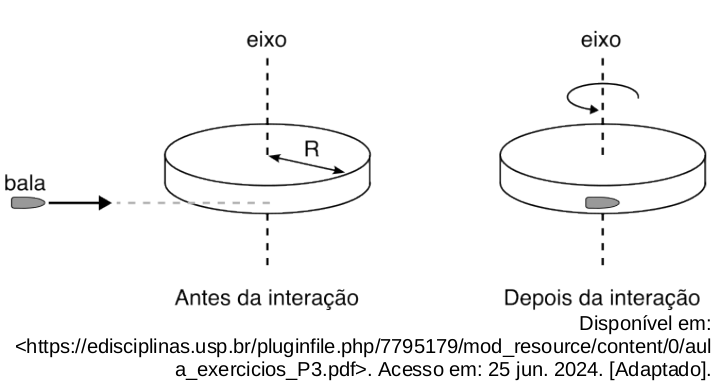
\includegraphics[width=0.8\textwidth]{figures/momento_angular.png}
\end{figure}

Uma bala de massa m se move horizontalmente com
velocidade v. A bala atinge a borda de um disco sólido, que
está inicialmente em repouso, ficando cravada nele (ver a
figura). O disco tem massa M, raio R, momento de inércia
$MR^{2}/2$ e está livre para girar em torno de seu eixo. Qual é a
velocidade angular do disco imediatamente após a bala ser
cravada nele?

\begin{itemize}
\item[(A)] $\Huge \omega = \frac{Mv}{(m+\frac{M}{2})R}$
\item[(B)] $\Huge \omega = \frac{mv}{(m+\frac{M}{2})R}$
\item[(C)] $\Huge \omega = \frac{mv}{(\frac{M}{2}-m)R}$
\item[(D)] $\Huge \omega = \frac{Mv}{(\frac{M}{2}-m)R}$
\end{itemize}

\vspace{0.5cm}

\textcolor{red}{\textbf{Solução:}}\\

\textbf{Princípio:}  
Como não há torques externos atuando em torno do eixo vertical, o momento angular do sistema em relação ao eixo é conservado.

\subsubsection*{Antes da colisão}
O momento angular do sistema em torno do eixo é apenas devido à bala:
\[
L_{\text{inicial}} = m v R
\]

\subsubsection*{Depois da colisão}
Após a colisão, a bala fica presa ao disco na borda, e o sistema (disco + bala) gira com velocidade angular \(\omega\).

Momento angular do disco:
\[
L_{\text{disco}} = I_{\text{disco}} \cdot \omega = \frac{1}{2} M R^2 \cdot \omega
\]

Momento angular da bala (considerada puntiforme a distância \(R\) do eixo):
\[
L_{\text{bala}} = m R^2 \cdot \omega
\]

Assim, o momento angular total após a colisão é:
\[
L_{\text{final}} = \left( \frac{1}{2} M R^2 + m R^2 \right) \omega
\]

\subsubsection*{Conservação do momento angular}
\[
L_{\text{inicial}} = L_{\text{final}}
\]

\[
m v R = \left( \frac{1}{2} M R^2 + m R^2 \right) \omega
\]

Dividindo ambos os lados por \(R\):
\[
m v = \left( \frac{1}{2} M + m \right) R \omega
\]

Isolando \(\omega\):
\[
\omega = \frac{m v}{R \left( \frac{1}{2} M + m \right)}
\]

\subsection*{Resposta final:}
\[
\boxed{
\omega = \frac{m v}{\left(m + \frac{1}{2} M\right)R}
}
\]

A resposta correta é alternativa \colorbox{green!50}{\textbf{B}}.
\end{flushleft}

\noindent\rule{\linewidth}{0.6pt}\\

\begin{flushleft}
\textbf{\textcolor{blue}{\Large Q38}}\\
\noindent
\colorbox{green!30}{Qual o astrônomo que propôs um modelo geocêntrico que
permitia descrever e prever} \colorbox{green!30}{as posições dos planetas e que, para isso, propôs que o movimento retrógrado dos planetas}
não tem sempre o mesmo aspecto e duração?

\begin{itemize}
\item[(A)] Galileu Galilei.
\item[(B)] Johannes Kepler.
\item[(C)] Cláudio Ptolomeu.
\item[(D)] Nicolau Copérnico.
\end{itemize}

\vspace{0.5cm}

\textcolor{red}{\textbf{Solução:}}\\

\section*{Resposta correta}

\[
\boxed{\text{(C) Cláudio Ptolomeu}}
\]

\section*{Explicação detalhada}

\subsection*{Quem foi Ptolomeu?}
Cláudio Ptolomeu foi um astrônomo, matemático e geógrafo grego que viveu em Alexandria, no Egito, no século II d.C. Ele escreveu a obra \textit{Almagesto}, que se tornou o principal tratado astronômico da Antiguidade e da Idade Média.

\subsection*{O que ele propôs?}
Ptolomeu refinou o antigo modelo geocêntrico (originalmente defendido por Aristóteles e Hiparco), criando um sistema geométrico e matemático capaz de:
\begin{itemize}
    \item Prever com precisão a posição dos planetas no céu em diferentes datas.
    \item Explicar por que os planetas às vezes parecem parar e andar para trás (\textit{movimento retrógrado aparente}).
\end{itemize}

\subsection*{Como ele explicou o movimento retrógrado?}
Para explicar o movimento retrógrado no \textbf{modelo geocêntrico}, Ptolomeu propôs que cada planeta não girava apenas em torno da Terra, mas fazia isso percorrendo duas trajetórias ao mesmo tempo:
\begin{itemize}
    \item Um \textbf{deferente}: círculo grande ao redor da Terra.
    \item Um \textbf{epiciclo}: círculo menor, cujo centro se move ao longo do deferente.
\end{itemize}

Esse sistema (\textit{deferente + epiciclo}) conseguia reproduzir as irregularidades do movimento dos planetas, inclusive o fato de que o movimento retrógrado não tinha sempre o mesmo tamanho nem a mesma duração para cada planeta.

\section*{Por que não as outras alternativas?}

\begin{itemize}
    \item \textbf{(A) Galileu Galilei}: Defendeu o heliocentrismo e fez observações com telescópio (\textit{séc. XVII}).
    \item \textbf{(B) Johannes Kepler}: Refinou o heliocentrismo com órbitas elípticas, rejeitando o geocentrismo (\textit{séc. XVII}).
    \item \textbf{(D) Nicolau Copérnico}: Propôs o heliocentrismo com órbitas circulares (\textit{séc. XVI}).
\end{itemize}

Somente \textbf{Ptolomeu} defendeu um modelo \textbf{geocêntrico}, consistente com as crenças da época, que já explicava as variações do movimento retrógrado.

\section*{Resumo}

\begin{center}
\small
\begin{tabular}{|c|c|c|}
\hline
\textbf{Astrônomo} & \textbf{Modelo} & \textbf{Movimento retrógrado} \\
\hline
\textbf{Ptolomeu} & Geocêntrico com epiciclos & Explicava corretamente o aspecto variável \\
\hline
Galileu & Heliocentrismo com telescópio & Observações em defesa do heliocentrismo \\
\hline
Kepler & Heliocentrismo com órbitas elípticas & Refinamento matemático \\
\hline
Copérnico & Heliocentrismo com órbitas circulares & Proposta inicial \\
\hline
\end{tabular}
\end{center}


A resposta correta é alternativa \colorbox{green!50}{\textbf{C}}.
\end{flushleft}

\noindent\rule{\linewidth}{0.6pt}\\

\section*{Gravitação Universal}

\textbf{Lei da Gravitação Universal:}
\begin{equation*}
  F = -G \frac{m_1 m_2}{r^2}
\end{equation*}

\textbf{Campo gravitacional:}
\begin{equation*}
  g = \frac{G M}{r^2}
\end{equation*}

\textbf{Energia potencial gravitacional:}
\begin{equation*}
  E_p = -\frac{G M m}{r}
\end{equation*}

\section*{Demonstração da Velocidade de Escape}

\colorbox{green!40}{A velocidade de escape é a mínima velocidade necessária para um corpo escapar da} \\
\colorbox{green!40}{gravidade de um planeta,} sem considerar resistência do ar.

\subsection*{Conservação de Energia}

Considerando um corpo de massa $m$ lançado da superfície de um planeta de massa $M$ e raio $R$:

\begin{itemize}
  \item Energia mecânica inicial:
  \[
  E_{\text{inicial}} = \frac{1}{2}mv^{2}_{e} - \frac{GMm}{R}
  \]
  \item Energia mecânica final (no infinito): 
  \[
  E_{\text{final}} = 0
  \]
\end{itemize}

Aplicando a conservação da energia:

\[
\frac{1}{2}mv^2_{e} - \frac{GMm}{R} = 0
\Rightarrow \frac{1}{2}v^2_{e} = \frac{GM}{R}
\Rightarrow v_{e} = \sqrt{\frac{2GM}{R}}
\]

\noindent
\textbf{Conclusão:} A velocidade de escape depende apenas da massa e do raio do corpo celeste, e não da massa do objeto lançado.

\noindent\rule{\linewidth}{0.6pt}\\

\begin{flushleft}
\textbf{\textcolor{blue}{\Large Questao 38}}\\
\noindent
Um foguete é lançado verticalmente para cima a partir da
superfície da Terra. Se a velocidade inicial do foguete for
metade da velocidade de escape da Terra, qual a altura que
o foguete atingirá, em unidades do raio da Terra (R$_{T}$)?
Despreze as influências da rotação da Terra no movimento
do foguete.

\begin{itemize}
\item[(A)] (7/3)R$_{T}$.
\item[(B)] (5/3)R$_{T}$.
\item[(C)] (2/3)R$_{T}$.
\item[(D)] (1/3)R$_{T}$.
\end{itemize}

\vspace{0.5cm}

\textcolor{red}{\textbf{Solução:}}\\

A energia mecânica total do foguete se conserva, pois desprezamos a resistência do ar.  
Na superfície da Terra (\(r = R_T\)), a energia total é a soma da energia cinética e potencial:  

\[
E_i = \frac{1}{2} m v_0^2 - \frac{G M_T m}{R_T}
\]

Na altura máxima (\(r = r_{\text{max}}\)), a velocidade do foguete é nula (\(v_f = 0\)):  

\[
E_f = 0 - \frac{G M_T m}{r_{\text{max}}}
\]

Conservação da energia mecânica: \(E_i = E_f\)  
Portanto:

\[
\frac{1}{2} m v_0^2 - \frac{G M_T m}{R_T} = - \frac{G M_T m}{r_{\text{max}}}
\]

Cancelamos \(m\) em todos os termos:

\[
\frac{1}{2} v_0^2 - \frac{G M_T}{R_T} = - \frac{G M_T}{r_{\text{max}}}
\]

Sabemos que a \textbf{velocidade de escape} é dada por:

\[
v_e = \sqrt{\frac{2 G M_T}{R_T}}
\]

Como a velocidade inicial do foguete é \(v_0 = \frac{v_e}{2}\), temos:

\[
v_0^2 = \left( \frac{v_e}{2} \right)^2 = \frac{v_e^2}{4} = \frac{1}{4} \cdot \frac{2 G M_T}{R_T} = \frac{G M_T}{2 R_T}
\]

Substituímos \(v_0^2\) na equação da energia:

\[
\frac{1}{2} \cdot \frac{G M_T}{2 R_T} - \frac{G M_T}{R_T} = - \frac{G M_T}{r_{\text{max}}}
\]

\[
\frac{G M_T}{4 R_T} - \frac{G M_T}{R_T} = - \frac{G M_T}{r_{\text{max}}}
\]

\[
-\frac{3}{4} \cdot \frac{G M_T}{R_T} = - \frac{G M_T}{r_{\text{max}}}
\]

Eliminamos o sinal e \(G M_T\):

\[
\frac{3}{4 R_T} = \frac{1}{r_{\text{max}}}
\]

Então:

\[
r_{\text{max}} = \frac{4}{3} R_T
\]

A altura máxima \(h_{\text{max}}\) acima da superfície é:

\[
h_{\text{max}} = r_{\text{max}} - R_T = \frac{4}{3} R_T - R_T = \frac{1}{3} R_T
\]

\section*{Resposta final:}

\[
\boxed{h_{\text{max}} = \frac{1}{3} R_T}
\]

O foguete atinge uma altura máxima igual a \(\frac{1}{3}\) do raio da Terra.


A resposta correta é alternativa \colorbox{green!50}{\textbf{D}}.
\end{flushleft}

\noindent\rule{\linewidth}{0.6pt}\\

\begin{flushleft}
\textbf{\textcolor{blue}{\Large Q39}}\\
\noindent
Um satélite de massa m orbita um planeta de massa M em
uma órbita circular de raio R. O tempo necessário para uma
volta completa do satélite em torno do planeta é

\begin{itemize}
\item[(A)] independente de M.
\item[(B)] proporcional a R$^{3/2}$.
\item[(C)] dependente de m.
\item[(D)] proporcional a R$^{2}$.
\end{itemize}

\vspace{0.5cm}

\textcolor{red}{\textbf{Solução:}}\\

A força gravitacional fornece a força centrípeta necessária:

\[
\frac{G M m}{R^2} = m \frac{v^2}{R}
\]

Cancelando \(m\) e resolvendo para \(v\):

\[
v = \sqrt{\frac{G M}{R}}
\]

O período \(T\) é dado por:

\[
T = \frac{2\pi R}{v}
\]

Substituindo \(v\):

\[
T =
\sqrt{\frac{4 \pi^{2} R^{3}}{G M}} =\sqrt{\frac{4 \pi^{2}}{G M}}\sqrt{R^{3}} = \sqrt{\frac{4 \pi^{2}}{G M}} R^{3/2}
\]


\section*{Resposta final:}

\[
\boxed{
T \propto R^{3/2}
}
\]


A resposta correta é alternativa \colorbox{green!50}{\textbf{B}}.
\end{flushleft}

\noindent\rule{\linewidth}{0.6pt}\\

\begin{flushleft}
\textbf{\textcolor{blue}{\Large Q40}}\\
\noindent
Uma função de estado de um sistema termodinâmico fica
completamente definida quando o estado do sistema é
especificado. Isso pode ser representado num diagrama
pressão-volume do sistema, que ilustra seus estados inicial
e final. Qual das grandezas abaixo é uma função de estado
de um sistema termodinâmico?

\begin{itemize}
\item[(A)] A energia interna.
\item[(B)] O calor.
\item[(C)] O trabalho.
\item[(D)] A massa.
\end{itemize}

\vspace{0.5cm}

\textcolor{red}{\textbf{Solução:}}\\

\section*{Introdução: Funções de Estado em Termodinâmica}

A Termodinâmica é a área da Física que estuda as transformações de energia e as propriedades macroscópicas da matéria, como temperatura, pressão e volume. Para descrever um sistema termodinâmico, é necessário especificar o \textbf{estado do sistema}, que é determinado por um conjunto de variáveis chamadas \textbf{variáveis de estado}.

Quando um sistema evolui de um estado inicial para um estado final, podemos calcular as mudanças sofridas em algumas grandezas físicas. Algumas dessas grandezas dependem apenas do estado inicial e final do sistema, enquanto outras dependem do caminho seguido durante o processo.

\subsection*{O que é uma função de estado?}

Uma \textbf{função de estado} é uma grandeza física cujo valor só depende do estado atual do sistema, isto é, das condições termodinâmicas (como \(P\), \(V\), \(T\), \(U\) etc.), e \textbf{não depende do processo pelo qual o sistema chegou a esse estado}.

Ou seja:
\begin{quote}
As funções de estado são propriedades macroscópicas que caracterizam completamente o estado do sistema. Sua variação entre dois estados é a mesma, independentemente do caminho percorrido entre eles.
\end{quote}

\subsection*{Exemplos clássicos de funções de estado:}
\begin{itemize}
    \item Energia interna (\(U\))
    \item Entalpia (\(H\))
    \item Entropia (\(S\))
    \item Pressão (\(P\))
    \item Volume (\(V\))
    \item Temperatura (\(T\))
\end{itemize}

Essas grandezas podem ser representadas em diagramas, como os famosos diagramas \(P \times V\) ou \(T \times S\), que ilustram estados e trajetórias de processos.

\subsection*{E o que não é função de estado?}

Grandezas como o \textbf{calor trocado} (\(Q\)) e o \textbf{trabalho realizado} (\(W\)) durante um processo dependem de 
como o sistema evoluiu — são chamadas de \textbf{funções de processo}.

Por exemplo: para comprimir um gás do volume \(V_1\) ao volume \(V_2\), o trabalho realizado pode ser maior ou menor 
dependendo do caminho seguido (isotérmico, adiabático etc.), mas a variação de energia interna só depende do estado inicial e final.

A resposta correta é alternativa \colorbox{green!50}{\textbf{A}}.
\end{flushleft}

\noindent\rule{\linewidth}{0.6pt}\\

\begin{flushleft}
\textbf{\textcolor{blue}{\Large Q41}}\\
\noindent
Uma bomba de calor serve para extrair calor do ambiente
externo a 7°C e aquecer o interior de uma casa a 27°C.
Considerando que a bomba é uma máquina de Carnot, para
cada 15.000 J de calor entregue dentro de casa, a menor
quantidade de trabalho que deve ser fornecido à bomba é

\begin{itemize}
\item[(A)] 2.500 J.
\item[(B)] 2.000 J.
\item[(C)] 1.500 J.
\item[(D)] 1.000 J.
\end{itemize}

\vspace{0.5cm}

\textcolor{red}{\textbf{Solução:}}\\

\section*{Definição}

Uma máquina térmica converte calor em trabalho, operando entre duas fontes térmicas.

\section*{Rendimento}

\[
\eta = \frac{W}{Q_q} = \frac{Q_q - Q_f}{Q_q} = 1 - \frac{Q_f}{Q_q}
\]

\begin{itemize}
  \item \( \eta \): rendimento
  \item \( W \): trabalho útil
  \item \( Q_q \): calor absorvido da fonte quente
  \item \( Q_f \): calor rejeitado à fonte fria
\end{itemize}

\section*{Rendimento da Máquina de Carnot}

\[
\eta_{\text{Carnot}} = 1 - \frac{T_f}{T_q}
\]

\subsection*{Calcular o rendimento da bomba de calor:}

\[
\eta = 1 - \frac{T_f}{T_q} = 1 - \frac{7^{\circ}\textrm{C} + 273\textrm{K}}{27^{\circ}\textrm{C}+ 273\textrm{K}} = 1 - \frac{280}{300} = 1 - 0.933333 = 0.066667 = 6.67\%
\]

Agora podemos calcular o trabalho realizado pela bomba de calor:

\[
  W = \eta Q_q = 6.67\% \times 15.000 \textrm{J} = 1.000 \textrm{J}
\]
A resposta correta é alternativa \colorbox{green!50}{\textbf{D}}.
\end{flushleft}

\noindent\rule{\linewidth}{0.6pt}\\

\section*{Princ\'ipios da Termodinâmica}

\subsection*{Primeiro Princípio}
\begin{equation*}
    \Delta U = Q - W   \hspace{0.5cm} \longrightarrow \hspace{0.5cm} Q = W + \Delta U
\end{equation*}
\subsection*{Segundo Princípio}
\begin{itemize}
    \item O calor não flui espontaneamente de um corpo frio para um corpo quente.
    \item Entropia tende a aumentar.
\end{itemize}

\section*{O que é entropia?}
A entropia (\(S\)) é uma função de estado que mede o grau de desordem de um sistema, a quantidade de microestados possíveis, e a irreversibilidade de processos.

\section*{Definição termodinâmica}
Para processos reversíveis:

\[
\Delta S = \int \frac{dQ_{\text{rev}}}{T}
\]

Para temperatura constante (isotérmico):

\[
\Delta S = \frac{Q_{\text{rev}}}{T}
\]

\section*{Segunda Lei da Termodinâmica}

\[
\Delta S_{\text{total}} \geq 0
\]

\begin{itemize}
  \item \( \Delta S_{\text{total}} = 0 \): processo reversível
  \item \( \Delta S_{\text{total}} > 0 \): processo irreversível
\end{itemize}

\section*{Entropia estatística (Boltzmann)}

\[
S = k_B \ln \Omega
\]

\begin{itemize}
  \item \( k_B = 1{,}38 \times 10^{-23} \, \text{J/K} \)
  \item \( \Omega \): número de microestados possíveis
\end{itemize}

\section*{Unidade}
Joules por Kelvin (J/K)

\section*{Exemplos onde a entropia aumenta}
\begin{itemize}
  \item Derretimento de gelo
  \item Expansão de gás
  \item Mistura de substâncias
\end{itemize}

\subsection*{Terceiro Princípio}
\begin{itemize}
    \item A entropia de um cristal perfeito é zero no zero absoluto $(0\,K)$.
\end{itemize}

\noindent\rule{\linewidth}{0.6pt}\\

\begin{flushleft}
\textbf{\textcolor{blue}{\Large Q42}}\\
\noindent
Um corpo de massa m com calor específico C à temperatura
de 500 K é colocado em contato com outro corpo de mesma
massa e mesmo calor específico à temperatura de 100 K. O
sistema é colocado dentro de uma caixa isolada
termicamente durante o processo. A variação da entropia do
sistema quando os blocos alcançam o equilíbrio térmico é

\begin{itemize}
\item[(A)] mCln 5.
\item[(B)] mCln 3.
\item[(C)] mCln(9/5).
\item[(D)] mCln(5/3).
\end{itemize}

\vspace{0.5cm}

\textcolor{red}{\textbf{Solução:}}\\

\section*{Variação de Entropia do Sistema}

\textbf{Dados do problema:}
\begin{itemize}
    \item Dois corpos idênticos: mesma massa \(m\) e mesmo calor específico \(C\)
    \item Temperatura inicial do corpo quente: \(T_q = 500\,\mathrm{K}\)
    \item Temperatura inicial do corpo frio: \(T_f = 100\,\mathrm{K}\)
    \item Caixa isolada termicamente (processo adiabático para o universo, mas irreversível para o sistema)
\end{itemize}

Queremos calcular a variação de entropia do sistema quando os corpos atingem o equilíbrio térmico.

\subsection*{Temperatura de equilíbrio}

Como os corpos têm mesma massa e mesmo calor específico, a energia perdida pelo quente é igual à energia ganha pelo frio. Assim, a temperatura de equilíbrio é a média aritmética:
\[
T_e = \frac{T_q + T_f}{2} = \frac{500 + 100}{2} = 300\,\mathrm{K}
\]

\subsection*{Variação de entropia de cada corpo}

Sabemos que a variação de entropia de um corpo com calor específico constante é dada por:
\[
\Delta S = mC \int_{T_i}^{T_f} \frac{dT}{T} = mC \ln\left( \frac{T_f}{T_i} \right)
\]

\textbf{Para o corpo quente:}
\[
\Delta S_q =
mC \ln\left( \frac{T_e}{T_q} \right) =
mC \ln\left( \frac{300}{500} \right) =
mC \ln(0{,}6)
\]

\textbf{Para o corpo frio:}
\[
\Delta S_f =
mC \ln\left( \frac{T_e}{T_f} \right) =
mC \ln\left( \frac{300}{100} \right) =
mC \ln(3)
\]

\subsection*{Variação de entropia total do sistema}

A variação de entropia total do sistema é a soma das variações de cada corpo:
\[
\Delta S_\text{total} =
\Delta S_q + \Delta S_f =
mC \ln(0{,}6) + mC \ln(3)
\]

Utilizando a propriedade dos logaritmos:
\[
\ln(0{,}6) + \ln(3) = \ln(0{,}6 \times 3) = \ln(1{,}8)
\]

Logo:
\[
\Delta S_\text{total} =
mC \ln(\frac{9}{5})
\]

\subsection*{Resposta final:}
\[
\boxed{
\Delta S_\text{total} =
mC \ln(\frac{9}{5})
}
\]



A resposta correta é alternativa \colorbox{green!50}{\textbf{C}}.
\end{flushleft}

\noindent\rule{\linewidth}{0.6pt}\\

\begin{flushleft}
\textbf{\textcolor{blue}{\Large Questao}}\\
\noindent

\begin{itemize}
\item[(A)] 
\item[(B)] 
\item[(C)] 
\item[(D)] 
\end{itemize}

\vspace{0.5cm}

\textcolor{red}{\textbf{Solução:}}\\


A resposta correta é alternativa \colorbox{green!50}{\textbf{...}}.
\end{flushleft}

\noindent\rule{\linewidth}{0.6pt}\\

\begin{flushleft}
\textbf{\textcolor{blue}{\Large Questao}}\\
\noindent

\begin{itemize}
\item[(A)] 
\item[(B)] 
\item[(C)] 
\item[(D)] 
\end{itemize}

\vspace{0.5cm}

\textcolor{red}{\textbf{Solução:}}\\


A resposta correta é alternativa \colorbox{green!50}{\textbf{...}}.
\end{flushleft}

\begin{flushleft}
\textbf{\textcolor{blue}{\Large Questao}}\\
\noindent

\noindent\rule{\linewidth}{0.6pt}\\

\begin{itemize}
\item[(A)] 
\item[(B)] 
\item[(C)] 
\item[(D)] 
\end{itemize}

\vspace{0.5cm}

\textcolor{red}{\textbf{Solução:}}\\


A resposta correta é alternativa \colorbox{green!50}{\textbf{...}}.
\end{flushleft}

\noindent\rule{\linewidth}{0.6pt}\\

\begin{flushleft}
\textbf{\textcolor{blue}{\Large Questao}}\\
\noindent

\begin{itemize}
\item[(A)] 
\item[(B)] 
\item[(C)] 
\item[(D)] 
\end{itemize}

\vspace{0.5cm}

\textcolor{red}{\textbf{Solução:}}\\


A resposta correta é alternativa \colorbox{green!50}{\textbf{...}}.
\end{flushleft}

\noindent\rule{\linewidth}{0.6pt}\\

\begin{flushleft}
\textbf{\textcolor{blue}{\Large Questao}}\\
\noindent

\begin{itemize}
\item[(A)] 
\item[(B)] 
\item[(C)] 
\item[(D)] 
\end{itemize}

\vspace{0.5cm}

\textcolor{red}{\textbf{Solução:}}\\


A resposta correta é alternativa \colorbox{green!50}{\textbf{...}}.
\end{flushleft}

\noindent\rule{\linewidth}{0.6pt}\\

\begin{flushleft}
\textbf{\textcolor{blue}{\Large Questao}}\\
\noindent

\begin{itemize}
\item[(A)] 
\item[(B)] 
\item[(C)] 
\item[(D)] 
\end{itemize}

\vspace{0.5cm}

\textcolor{red}{\textbf{Solução:}}\\


A resposta correta é alternativa \colorbox{green!50}{\textbf{...}}.
\end{flushleft}

\begin{flushleft}
\textbf{\textcolor{blue}{\Large Questao}}\\
\noindent

\begin{itemize}
\item[(A)] 
\item[(B)] 
\item[(C)] 
\item[(D)] 
\end{itemize}

\vspace{0.5cm}

\textcolor{red}{\textbf{Solução:}}\\


A resposta correta é alternativa \colorbox{green!50}{\textbf{...}}.
\end{flushleft}

\noindent\rule{\linewidth}{0.6pt}\\

\begin{flushleft}
\textbf{\textcolor{blue}{\Large Questao}}\\
\noindent

\begin{itemize}
\item[(A)] 
\item[(B)] 
\item[(C)] 
\item[(D)] 
\end{itemize}

\vspace{0.5cm}

\textcolor{red}{\textbf{Solução:}}\\

A resposta correta é alternativa \colorbox{green!50}{\textbf{...}}.
\end{flushleft}

\noindent\rule{\linewidth}{0.6pt}\\

\begin{flushleft}
\textbf{\textcolor{blue}{\Large Questao}}\\
\noindent

\begin{itemize}
\item[(A)] 
\item[(B)] 
\item[(C)] 
\item[(D)] 
\end{itemize}

\vspace{0.5cm}

\textcolor{red}{\textbf{Solução:}}\\


A resposta correta é alternativa \colorbox{green!50}{\textbf{...}}.
\end{flushleft}

\noindent\rule{\linewidth}{0.6pt}\\

\begin{flushleft}
\textbf{\textcolor{blue}{\Large Questao}}\\
\noindent

\begin{itemize}
\item[(A)] 
\item[(B)] 
\item[(C)] 
\item[(D)] 
\end{itemize}

\vspace{0.5cm}

\textcolor{red}{\textbf{Solução:}}\\

A resposta correta é alternativa \colorbox{green!50}{\textbf{...}}.
\end{flushleft}

\noindent\rule{\linewidth}{0.6pt}\\

%%%%%%%% Bibliography 
% Os comandos para incluir as referências bibliográficas
%\printingbibliography

\end{document}
